\section{A photo trip to Sic Semper Tyrannis}
    \margininbox{At World's End}{
                    \begin{itemize}
                        \item Rhys Tyers
                        \item Tanguy Racine
                    \end{itemize}}{\explo}
                    
    The breeze made the leaves rustle, their shadows dancing on the white carbonate sand. The air was cooler by the \passage[river]{So\v{c}a} river, and the sound of merry children splashing about in their inflatable dinghies upstream was a welcome change from the \passage{Bivi} conversations.
    
    \bignote{After the desolation of the windswept, grey skies of the plateau, I thought it was time to come back down in the valley and enjoy the grapefruit beers and meaty pizza}. The sun was a nice addition too, so Jarv drove a team of us to \passage{Most Na So\v{c}i}, where the \passage[river]{Idrijca} river joined the \passage[river]{So\v{c}a}. The beers were left in the cold water while I blew air into side compartments the boat.
    
    I enjoyed then a few rides on the river, mainly trying to enforce coordination in the paddling, which enabled Rhys and I to turn the boat round and maintain our position with synchronised movements, prow against the current. The beauty and complexity of the manoeuvre was lost on the bystanders unfortunately so we ran our proud ship aground lower downstream and carried the boat back to the take off. Then I sat on my towel and enjoyed the sight.


\begin{marginsurvey}
	\includegraphics[width= \linewidth]{"images/little_insets/touching_the_void_inset".pdf}
	\caption[Davy Jones' Locker]{Plan view of the passages below \protect\passage{Sic Semper Tyrannis} --- Slovenian National Grid EPSG 3794}
\end{marginsurvey}


    After a moment I spoke with Rhys.
    `There are very few photos of the southern extensions of the system' he remarked. There was a faint smile on his face, and his eyebrow travelled up his forehead.  That was true. 

`You intend to take some?'

    `Probably.. Yes'.

    `How was the pushing with Ben' How about the pitch you found' Does it go?' I replied.

    `We followed the water from Sic Semper Tyrannis, and stopped at a pitch...yes, that would be a good trip wouldn't it?'

    `Yes, go down, photograph then push. I'm interested in this business of taking photos of Helm's Deep chamber and the rest, it could be impressive'

    `Sure, RT and TR again'

    `Count me in then!' I said, looking at the blue green waters rushing by. On the morrow, we bid farewell to \passage{Tolmin} and ascended to the plateau once again. The weather turned, temperatures rose, and the sun came out as Rhys and I prepared our kit.\sidenote{Editor's note: This is only the author's reproduction of a half-forgotten conversation. Rhys Tyers doesn't actually use this syntax in speech.}
    
    \mydelimiter

    Two days later, we were descending to \passage{X-Ray} with a good plan, three nights, two pushing trips. The first would be to \passage{Atlantis} and its extensions, to document the finds from the last three years with photographs.

    We started the photo session at the \passage{Red Baron} chamber traverse, and worked our way to \passage{Stuck in Paradise}. After the pitch, some quick photographs of the \passage{Atlantis} stalactites saw us reach \passage{Helm's Deep} chamber. A rope led up to \passage{Touching the Void}, at the top of a loose rubble slope, underneath a fallen slab of white limestone. Ascending up there I gained a good view of the chamber some 20 metre higher than Rhys. I slid underneath the slab and carried on climbing, until I popped out onto a pitch head. Water from two streams could be seen joining into a waterfall, and a climb up led to another vantage point overlooking the pitch. The top of the pitch was again a loose slope, disappearing into the darkness above. A lead for bolt climbers which could be reached by traversing over the rock bridge I stood on, then over the drop, and further up still for another 15\,m.

	\bignote{The sight of the water however reminded us that exploration needs to be thorough, as well as exciting. Caver legends such as Norbert Casteret were, after all, hydrogeologists as well as speleologists}. Where did that water go' Where did it come from' The former question was more easily answered, so we climbed down to the bottom of \passage{Helm's Deep} chamber, where an opening in the slope led to a water chamber of modest dimensions.
    \begin{survey}[b!]
        \checkoddpage \ifoddpage \forcerectofloat \else \forceversofloat \fi
        \centering
        \frame{\includegraphics[width=\linewidth]{"images/2015/tanguy-photography-2015/helmsdeep".png}}

        \caption[Touching the Void - grade 1]{An extended elevation view of \protect\passage{Helm's Deep} chamber and adjoining \protect\passage{Touching the Void} extensions \pen{Rhys Tyers, underground logbook}}
        \label{helms deep}
         
    \end{survey}

    \begin{figure*}[t!]
        \checkoddpage \ifoddpage \forcerectofloat \else \forceversofloat \fi
        \centering
        \begin{subfigure}[t]{0.68\textwidth}
            \centering
            \frame{\includegraphics[width=\linewidth]{"images/2015/tanguy-photography-2015/belowhelm_sdeep".jpg}}
            \caption{}\label{water chamber below helm's deep}
        \end{subfigure}
        \hfill
        \begin{subfigure}[t]{0.303\textwidth}
            \centering
            \frame{\includegraphics[width=\linewidth]{"images/2015/tanguy-photography-2015/rhystyers_sic_semper__1_".jpg}}
            \caption{} \label{HelmsDeep}
        \end{subfigure}

        \vspace{0.3cm}
        
        \begin{subfigure}[t]{\textwidth}
            \centering
            \frame{\includegraphics[width=\linewidth]{"images/2015/tanguy-photography-2015/rhystyers_touching_the_void__1_".jpg}}
            \caption{} \label{Touching the Void 1}
        \end{subfigure}
        
        \caption{
            \emph{a} Water chamber below \protect\passage{Helm's Deep}
            \emph{b} In \protect\passage{Helm's Deep} chamber
            \emph{c} The top of the climb in \protect\passage{Touching the Void}, where a 30m pitch takes in the active waterfall \pic{Rhys Tyers}
        }
    \end{figure*}

    A small stream emerged from an obscure fissure which enlarged to an anthropic opening on top. Rhys climbed up into the rift a metre above the water and followed the passage leading off upstream. At every meander, sharp prongs of rock remained, catching on our suits, forcing us to negotiate the climb with care. A few twists and turns followed, until a flat out, damp crawl connected with the base of a large pitch. The rumble of the water rushing down resonated all around, and a slight drizzle dusted Rhys's shoulders with glittering droplets. This was the bottom of the two-waterfall pitch, underneath the pile of  cave sediment that make the floor of \passage{Helm's Deep} chamber.

    \begin{figure*}[t!]
        \checkoddpage \ifoddpage \forcerectofloat \else \forceversofloat \fi
        \centering
        \frame{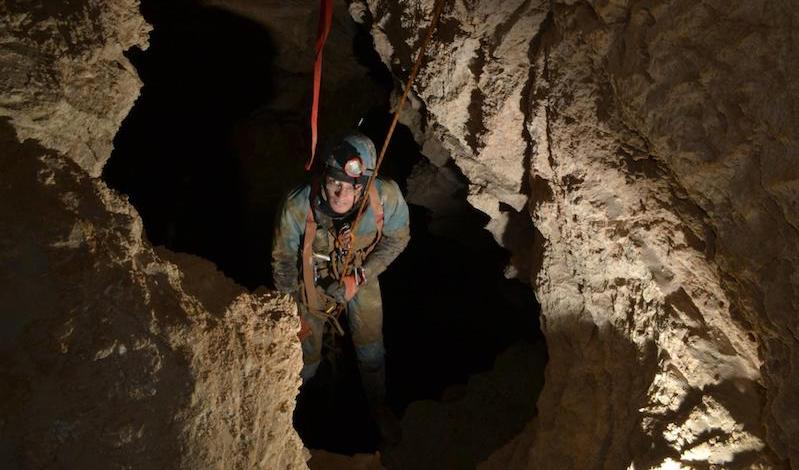
\includegraphics[width=\textwidth]{images/2015/tanguy-photography-2015/worldsend2015.jpg}}
        
        \caption{The fossil pitch named `\protect\passage{At Worlds End}' which is found downstream of the \protect\passage{Sic Semper Tyrannis} \pic{Rhys Tyers}}
        \label{water chamber below helm's deep}
    \end{figure*}



	The first piece of the puzzle fell into place. Back at the water chamber, we could see the stream disappearing into a tube. This almost certainly leads to the lower water chamber which is the termination of \passage{Sic Semper Tyrannis}. In the latter, the water flows underneath boulders to \passage{Davy Jones' Locker} passage. Swiftly, we caved towards the pushing front, trying to piece together the hydrology of this region of cave.



 Following the water, past the sump bypass flat out crawl, to the undescended pitch Rhys and Ben had found earlier. At the head, I put in a bolt, backed-up by two sling anchors and tied up a Y-hang knot. When I looked at the remaining length of rope available to descend, I let out a loud curse. Either rope we'd brought was too short on its own after the knots were tied.

    I had learned how tie two ropes together beforehand; whether I'd trust my life with it was another matter. After a few minutes deliberating however, we'd satisfied ourselves that if it had been done to descend `\passage{Godzilla}', with not one, or two, but three knots, then surely it could be done again. Not that our own pitch was such a monster, but soon after the take off, the pitch belled out, and after the knot pass, a smooth descent brought me on top of a boulder pile, in a dry chamber. Rhys came down soon after. There was no obvious way on, though the rumble of water could be heard, so we searched for man sized openings between the carefully positioned boulders. Dropping down a few metres brought us to a tight rift, heading west. 10 metres further, the rift opened onto a small balcony overlooking a sizeable pitch, where the sound from a cascading streamway could be heard. To our left, the spray from the \passage{Davy Jones' Locker} almost reached us, while to the right, the morphology of the pitch suggested a far larger inlet of water down below.



%    \begin{figure*}[t!]
    %    \checkoddpage \ifoddpage \forcerectofloat \else \forceversofloat \fi
     %   \centering
       % \begin{subfigure}[t]{0.41\textwidth}
          %  \centering
            %\frame{\includegraphics[width=\linewidth]{"images/2015/tanguy-photography-2015/davy_jones_locker".jpg}}
       %     \caption{}\label{davyjones}
     %   \end{subfigure}
     %   \hfill
    %    \begin{subfigure}[t]{0.58\textwidth}
       %     \centering
         %   \frame{\includegraphics[width=\linewidth]{"images/2015/tanguy-photography-2015/extended_elevation_worlds_end".jpg}}
         %   \caption{} \label{helmsdeep}
      %  \end{subfigure}

   %     \caption{
      %      \emph{(a)} \protect\passage{Davy Jones' Locker} grade 1 plan survey
        %    \emph{(b)} In \protect\passage{Helm's Deep} chamber grade 1 extended elevation --- scanned, Rhys Tyers
     %   }
  %  \end{figure*}
    


    We were running out of rope and time so we left this last piece of the puzzle for another time. It is probable that the larger inlet is the water from \passage{Brezno Slapov}, and that the water we followed came down in one of the wet avens of \passage{Lethe}. Only descending the pitch would prove it, but nonetheless, it was satisfying for us to solve one small mystery of \passage{Sysmig}. \name{Tanguy Racine}
    
\clearpage

   \fullwidthbox{Andrea Bocelli --- Heading towards the Old System}{
                    Booze, dope, woman. Such a perfect day.
                    After that endless 230\,m of passage we bolted a traverse across a pitch (not pushed, too wet), we found another 20\,m of that passage which ended in a... hmmm... prelom? Full of water. It continues in the same direction (N-> S) on at least two levels. We pushed some 50\,m but stopped before a small pitch because we left the gear behind. There you can hear water around the corner. We returned to the gear in the big “prelom” and followed the water. We made a descent (cc 30\,m) turned back south and squeezed through a needle hole and came to a big pitch (30\,m+). We could not see the bottom. We only had 15m of rope which we left on an anchor. Then we turned back and lived happily ever after.
                    O, jeah [sic] ... no surveying today. At least 5 times more water than yesterday !! Still we would like the last pitch we found to be named `Time to say Goodbye'. \name{Grega Maffi}
                    In life we must do only one thing: die. So, who the hell came up with caving? \name{Tja\v{s}a Rutar} }    
    
    \section{A new lead in the north}
\margininbox{Lazarus}{
     \begin{citemize}
    \item Rhys Tyers
    \item Tanguy Racine
    \end{citemize}}{\explo}
    
It was three weeks in the expedition, I'd had a break in \passage[town]{Tolmin}, and was about to set off for a photo-trip with Rhys to \passage{Sic Semper Tyrannis}, followed by a visit to the northern reaches of the system and maybe \passage[sump]{Colarado Sump}. The bivi was full of cavers, some actively descending surface shafts nearby, others keen to dig \passage[cave]{K12}. I had a plan to make the washing area somewhat salubrious again. Decades worth of edible matter had piled up over the scree, and penetrated deep underneath the rock cover, slowly turning to an impermeable layer of miasma clogging up the interstices between the cobbles.

It was decided that a good way of draining the water from this area where, after all, mess tins and cutlery were supposed to be cleaned, was to dig a deep trench, removing scree and sediment alike, and to fill the space with fresh scree. I took a shovel, a digger's jerrycan (the lateral face being cut out to resemble a miner's waggon) and a tacklesack. 

Getting the first inches of depth was hard work, filling the tacklesack half-way up, carrying it out of the bivi, and starting again. Very quickly, a foul stench emanated from the hole, hydrogen sulphide from decomposing matter. On the way, I unearthed some old bits of tat and string along with a healthy dose of coal-black slime. After fifteen tacklesacks or so, the hole had a capacity of almost 100\,L. I stopped then, as the sun beat down on the hole, giving the vapours an even fouler smell. I also had to prepare for the underground trip, but secretly hoped to get back to it later...

 \begin{marginfigure}
\checkoddpage \ifoddpage \forcerectofloat \else \forceversofloat \fi
\centering
 \frame{\includegraphics[width=\linewidth]{"images/2015/tanguy-lazarus-2015/smash-jarv-rhys".jpg}} 
 \caption{Rhys Tyers picking his way through the complex boulder choke of \protect\passage{Smash} \pic{Jarvist Frost}}
 \label{smash}
\end{marginfigure}

`I'm quite excited about visiting the northern bits of the cave' I told Rhys as I put my wet socks on. The camp was silent, even \passage{Zimmer} could not be heard which meant it was dry on top of the mountain. Oversuit, SRT kit, helmet. A last check and we blew the candles, squeezed the rubber duck and left the shadowy alcove where the tent was pitched.

I descended \passage{Big Rock Candy Mountain} and followed Rhys to \passage{Playboy Junction}, through the \passage{Leprechaun series}, down \passage{Memory Lane} to \passage[camp]{Red Cow} camp. From then on, it was discovery for me, in the dry sandy passages of \passage{No More Potatoes}. On the way, Rhys pointed out a rope disappearing up an aven `\passage[aven]{Strap on the Nitro}' he said. Without further ado, we went through a pebbly crawl, up a very long slope, culminating at the start of \passage{Smash}, a series of breakdown chambers connected by free climbs. Thanks to Rhys's route-finding, we soon broke into Miles Underground, a spacious rift with a boulder floor. This passage was very reminiscent of Wales caving, especially the entrance to \passage[not a real cave]{Ogof Ffynnon Ddu}.

Soon, Rhys spotted a gap in between boulders from which a small stream emerged. The stream almost immediately dropped into a clean washed chamber. From an alternate route, we made our way down into the water chamber, where a rift in the far wall could be seen to swallow the stream whole. We cautiously had a peek from the top of the drop, and decided it was a promising lead, got busy putting a bolt and tied in a Y-hang. This time I let Rhys descend first. While the higher section of the 15\,m drop was rigged well away from the water, the bottom third was exposed to the drips, which pooled at the base of the rope. A quick abseil from both of us meant we stayed relatively dry but to our dismay the passage closed down almost immediately. 

I prussicked back up and waited for Rhys, who on his way up scouted for a higher traverse and possible lead. After spotting a likely alcove towards the top, he proceeded to reach it by bridging the rift. When that technique failed, he resorted to swinging across, but the rope was dangerously close to the wall so it was abandoned.

\begin{marginfigure}
\checkoddpage \ifoddpage \forcerectofloat \else \forceversofloat \fi
\centering
 \frame{\includegraphics[width=\linewidth]{"images/2015/tanguy-lazarus-2015/tanguy-bolting-worlds_end".jpg}} 
 \caption{Tanguy Racine driving a spitz in the hard limestone wall - although lightweight, the complete handbolting kit comprises hammer, driver, spanner, spitz, hangers, cones and maillons - it's easy to forget one item! \pic{Rhys Tyers}}
 \label{tanguy bolting}
\end{marginfigure}


We left it at that and continued our route northward to the very end of dry exploration: at \passage[duck]{Colarado Sump}, which had recently been passed by Jarvist Frost and Connor Roe.  Just before the silt banks that herald the end, Rhys took a turn to the right to have a quick look at the \passage{Hoover Dam} lead, a sizeable aven with numerous holds. It was no surprise that Connor had gotten quite high before turning round. At the bottom of the aven through, Rhys then spotted a cleft in the wall, `a true \emph{chattière}' he exclaimed.

`I bet it's been looked at before' Rhys exclaimed, `but let's have make sure nonetheless'. Soon we were both on our hands and knees, crawling up. The bowel did not close down immediately, and after ten metres it really looked like a small tube, connecting two large passages. Things were looking up, and we switched places so I could lead as well. After a sharp turn, the passage dropped into an incredibly tight rift. I reckoned that I could fit through the slot without SRT kit and any regard for personal safety but we turned around, and left this thirty metre long tube unsurveyed. 

I was caught short then and \bignote{it became evident that I'd contracted a gut disease whilst digging the trench in the Bivi. Finding a suitably dark corner, I let the tide wash over the rocks}. 

Rhys and I then had a look at the duck, going as far as the now well trodden silt banks. We turned around, climbed the smooth bedding plane to \passage[aven]{Infinity and Beyond} junction, whereupon we tried to reach a greater height in the aven. After reaching a suitably exposed vantage point, we decided not to put ourselves in an unnecessarily dangerous situation, and climbed back down. As if to comfort us in this decision, one of my footholds gave way and I slid two metres down the rift, back against a muddy slope. Rhys was well out of the way, but it served to remind us not to trust the rock anywhere. Caves are after all a hostile environment. 

Our spirits were somewhat dampened. Were there any more long horizontal offshoots to be found far below \passage[mountain]{Migovec}? We started the long trudge back up to \passage{Smash} with heavy hearts.

As we were approaching the start of the \passage{Smash} breakdown, Rhys climbed up on the western side of the boulder slope and cursed as the way on could not be found. Instead, a seemingly insignificant alcove opened underneath a protruding knob of rock. A small pit could be seen beyond. `Probably doesn't go anywhere right, ...right?'. I did not answer straight away, I looked at the beckoning darkness.

Slowly I undid the straps from my tacklesack and left it on the rocks. I jumped into the small  pit, at the bottom of which a tight flat out crawl led off. A few potato sized rocks lay here and there along the plane of bedding, which I shoved across. The crawl carried on downwards for five metres, beyond which I could not see a continuation. The plane disappeared underneath a floor of small pebbles, sloping in the opposite direction. `There nothing here' I said, but I didn't wait for a response: as soon as the words came out, they reverberated across the plane, amplified. `Wait?' I hummed loudly to ascertain that there was a great resonance in the passage. `There's an echo, there must be something beyond!'.
\begin{marginfigure}
	\checkoddpage \ifoddpage \forcerectofloat \else \forceversofloat \fi
	\centering
	\frame{\includegraphics[width=\linewidth]{"images/2015/tanguy-lazarus-2015/rhys-near-duck".jpg}} 
	\caption{Rhys Tyers near \passage{Colarado Sump} in a large phreatic trunk route \pic{Jarvist Frost}}
	\label{near duck}
\end{marginfigure}


I crept forward and extended my neck and saw what I had missed: an anthropic opening, and void space beyond. 

`I'm going to dig a few of the pebbles and then go through, take the instruments' I instructed excitedly. `Really, Are you sure it's worth it?' came the answer. 

I grabbed pebbles by the handful and dug a way through. Two minutes later I stood on virgin passage in a modest chamber with a rounded vault of solid rock. When Rhys emerged we shook hands on the discovery. At the far end of the chamber, the ceiling came down to meet the white sandy floor. A small opening led to a squeeze I asked Rhys to attempt first. 

After he went through I followed, with my chest compressed by a nodule of rock in the middle of the constriction. The rest of the body followed, and we stood in a second chamber, very similar in its shape. Going further along, we were faced with a pebbly dig. A small air opening perhaps ten centimetres high was spotted and Rhys insisted we start digging it out.
\begin{pagefigure}
	\checkoddpage \ifoddpage \forcerectofloat \else \forceversofloat \fi
	\centering
\frame{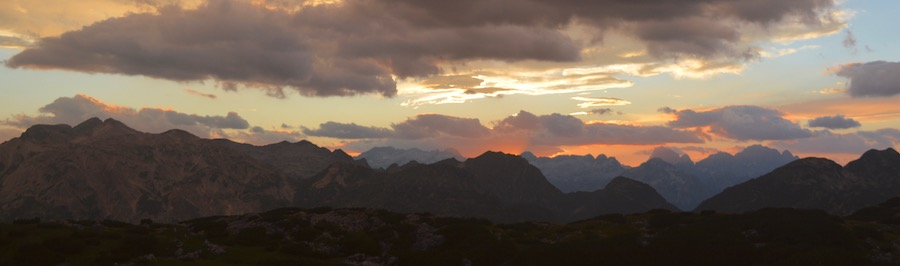
\includegraphics[width = \textwidth]{images/2015/tanguy-lazarus-2015/sunset_krn.jpg}}
\caption{We got out to another gorgeous sunset over \protect\passage{Krn} \pic{Tanguy Racine}} \label{fig:krn_sunset}
\end{pagefigure}

He persuaded me to give it a real go, as it was draughting significantly, so we carried on digging the sand and pebbles until the opening was passable. Rhys attempted it first and I followed. The ceiling was still low, and the way on was through tight passage on pristine sandy sedimentary formations where the small drips had collected into ephemeral streams. We crawled some more, carefully avoiding the stream and deeply conscious of the damage we were inflicting on this hitherto undisturbed sandy bank. Finally, we emerged into a third chamber of bigger dimensions, a storming lead! 

\begin{survey}[t!]
	\checkoddpage \ifoddpage \forcerectofloat \else \forceversofloat \fi
	\centering
	\frame{\includegraphics[width=\linewidth]{"images/2015/tanguy-lazarus-2015/lazarus".png}} 
	\caption[Lazarus (grade 1)]{A plan view of \passage{Lazarus} -\pen{Tanguy Racine,underground logbook}}
	\label{lazarus plan}
\end{survey}

We stopped there \sidenote{A stop on nothing. I regret it because we haven't come bakc}: I wanted to give us a reason to come back to this lead the following year. Rhys came round to my opinion and we surveyed back to \passage{Miles Underground} passage. This new lead headed towards the north west, and looked morphologically separate from the main rift leading to \passage{Colarado Sump}. Where would it go?


\name{Tanguy Racine}



